\section{Untangling feature magnitude and location}
\label{sec-where-info}
The convolutional layers preserve the coarse spatial layout of the network's input.
By layer conv-5, the original $227 \times 227$ input image has been progressively downsampled to $6 \times 6$.
This feature map is also sparse due to the $\max(x, 0)$ non-linearities used in the network (conv-5 is roughly 27\% non-zero; sparsity statistics for all layers are given in Table \ref{table:sparse}).
Thus, a convolutional layer encodes information in terms of (1) which filters have non-zero responses, (2) the magnitudes of those responses, and (3) their spatial layout.
In this section, we experimentally analyze the role of filter response magnitude and spatial location by looking at lesion studies on classification and detection tasks.

\begin{figure}[t!]
\centering
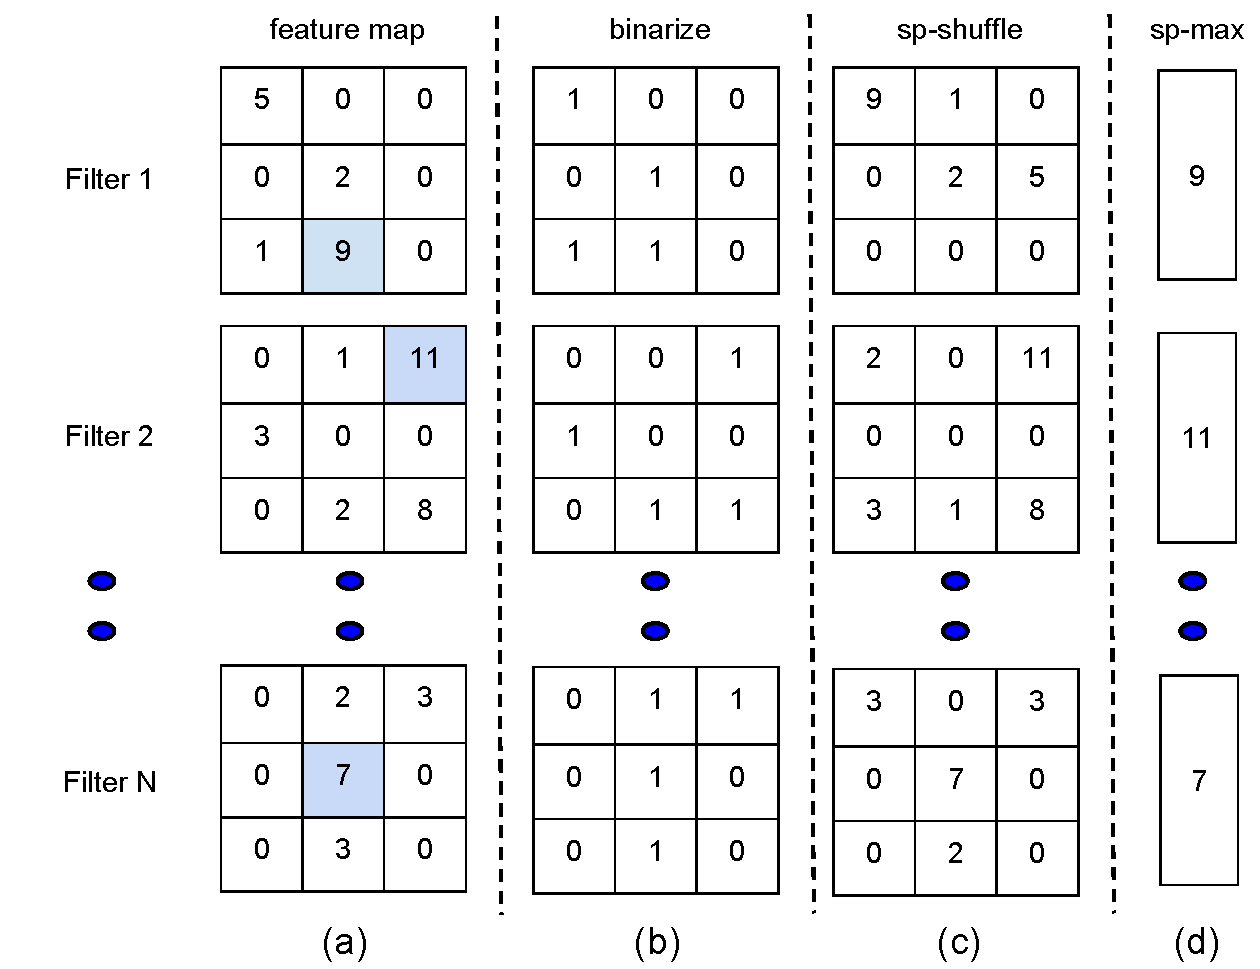
\includegraphics[height=6.5cm]{images/ablation.pdf}
\caption{Illustrations of ablations of feature activation spatial and magnitude information.
See Sections \ref{sub:imp-mag} and \ref{sub:imp-loc} for details.}
\label{fig:features}
\end{figure}

\subsection{How important is filter response magnitude?}
\label{sub:imp-mag}
\setlength{\tabcolsep}{4pt}
\begin{table}[t!]
\begin{center}
%\caption{Percentage non-zeros (sparsity) in filter responses of various layers of CNN.}
\caption{Percentage non-zeros (sparsity) in filter responses of CNN.}
\label{table:sparse}
\scalebox{1}{
\begin{tabular}{c|c|c|c|c|c|c}
conv-1 & conv-2 & conv-3 & conv-4 & conv-5 & fc-6 & fc-7 \\
\hline
$87.5 \pm 4.4$ & $44.5 \pm 4.4$ & $31.8 \pm 2.4$ & $32.0 \pm 2.7$ & $27.7 \pm 5.0$ & $16.1 \pm 3.0$ & $21.6 \pm 4.9$ \\
\end{tabular}}
\end{center}
\end{table}
\setlength{\tabcolsep}{1.4pt}

We can asses the importance of magnitude by setting each filter response $x$ to 1 if $x > 0$ and to $0$ otherwise. This binarization is performed prior to using the responses as features in a linear classifier and leads to loss of information contained in the magnitude of response while still retaining information about which filters fired and where they fired. 
In Tables \ref{table:class-ablation} and \ref{table:det-ablation} we show that binarization leads to a negligible performance drop for both classification and detection. 

For the fully-connected layers (fc-6 and fc-7) PASCAL-CLS performance is nearly identical before and after binarization.
This is a non-trivial property since transforming traditional computer vision features into short (or sparse) binary codes is an active research area. Such codes are important for practical applications in large-scale image retrieval and mobile image analysis \cite{gong2011iterative,weiss2009spectral}. Here we observe that sparse binary codes come essentially ``for free'' when using the representations learned in the fully-connected layers.

\subsection{How important is response location?}
\label{sub:imp-loc}
Now we remove spatial information from filter responses while retaining information about their magnitudes. We consider two methods for ablating spatial information from features computed by the convolutional layers (the fully-connected layers do not contain \emph{explicit} spatial information).

The first method (``sp-max'') simply collapses the $p \times p$ spatial map into a single value per feature channel by max pooling. The second method (``sp-shuffle'') retains the original distribution of feature activation values, but scrambles spatial correlations between columns of feature channels. To perform sp-shuffle, we permute the spatial locations in the $p \times p$ spatial map. This permutation is performed independently for each network input (i.e., different inputs undergo different permutations). Columns of filter responses in the same location move together, which preserves correlations between features within each (shuffled) spatial location. These transformations are illustrated in Figure \ref{fig:features}.

For image classification, damaging spatial information leads to a large difference in performance between original and spatially-ablated conv-1 features, but with a gradually decreasing difference for higher layers (Table \ref{table:class-ablation}). 
In fact, the performance of conv-5 after sp-max is close to the original performance. 
This indicates that a lot of information important for classification is encoded in the activation of the filters and not necessarily in the spatial pattern of their activations.
Note, this observation is not an artifact of small number of classes in PASCAL-CLS. On ImageNet validation data, conv-5 features and conv-5 after sp-max result into accuracy of 43.2 and 41.5 respectively. 
However, for detection sp-max leads to a large drop in performance. 
This may not be surprising since detection requires spatial information for precise localization.

\setlength{\tabcolsep}{4pt}
\begin{table}[t!]
\begin{center}
%\caption{Location and magnitude ablation study on PASCAL-CLS.}
\caption{Effect of location and magnitude feature ablations on PASCAL-CLS.}
\label{table:class-ablation}
\begin{tabular}{lccccc}
\noalign{\smallskip}
layer & no ablation (mAP) & binarize (mAP) & sp-shuffle (mAP) & sp-max (mAP) \\
\noalign{\smallskip}
\hline
\noalign{\smallskip}
conv-1 & $25.1 \pm 0.5$ & $17.7 \pm 0.2$ & $15.1 \pm 0.3$ & $25.4 \pm 0.5$  \\ 
conv-2 & $45.3 \pm 0.5$ & $43.0 \pm 0.6$ & $32.9 \pm 0.7$ & $40.1 \pm 0.3$  \\ 
conv-3 & $50.7 \pm 0.6$ & $47.2 \pm 0.6$ & $41.0 \pm 0.8$ & $54.1 \pm 0.5$  \\
conv-4 & $54.5 \pm 0.7$ & $51.5 \pm 0.7$ & $45.2 \pm 0.8$ & $57.0 \pm 0.5$  \\
conv-5 & $65.6 \pm 0.6$ & $60.8 \pm 0.7$ & $59.5 \pm 0.4$ & $62.5 \pm 0.6$  \\
fc-6   & $71.7 \pm 0.3$ & $71.5 \pm 0.4$ &  -             &  -   \\
fc-7   & $74.1 \pm 0.3$ & $73.7 \pm 0.4$ &  -             &  -   \\
\end{tabular}
\end{center}
\end{table}
\setlength{\tabcolsep}{1.4pt}

\setlength{\tabcolsep}{4pt}
\begin{table}[t!]
\begin{center}
\caption{Effect of location and magnitude feature ablations on PASCAL-DET.}
\label{table:det-ablation}
\scalebox{1.0}{
\begin{tabular}{l|c|c|c}
& no ablation (mAP) & binarize (mAP) & sp-max (mAP) \\
\hline
conv-5 & 47.6 & 45.7 & 25.4 
\end{tabular}}
\end{center}
\end{table}
\setlength{\tabcolsep}{1.4pt}

\begin{comment}
\setlength{\tabcolsep}{1pt}
\begin{table}[t!]
\begin{center}
\caption{Ablation study on PASCAL-DET using conv-5 features. Feature binarization leads to negligible drop in performance whereas as sp-max causes a large drop.}
\label{table:det-ablation}
\scalebox{0.70}{
\begin{tabular}{l|cccccccccccccccccccc||c}
\noalign{\smallskip}
& aero & bike & bird & boat & bottle & bus & car & cat & chair & cow & table & dog & horse & mbike & person & plant & sheep & sofa & train & tv & mAP \\
\noalign{\smallskip}
\hline
conv-5  & 57.8 & 63.9 & 38.8 & 28.0 & 29.0 & 54.8 & 66.9 & 51.3 & 30.5 & 52.1 & 45.2 & 43.2 & 57.3 & 58.8 & 46.0 & 27.2 & 51.2 & 39.3 & 53.3 & 56.6 & 47.6 \\
binarize & 57.9 & 61.3 & 32.6 & 24.7 & 27.5 & 55.0 & 64.7 & 49.8 & 25.3 & 47.4 & 44.5 & 40.3 & 54.6 & 56.4 & 43.6 & 27.1 & 48.4 & 41.6 & 54.3 & 57.6 & 45.7 \\
sp-max & 35.0 & 38.7 & 17.3 & 16.9 & 13.9 & 38.4 & 45.6 & 29.2 & 11.0 & 20.2 & 21.0 & 23.5 & 27.2 & 37.0 & 20.5 & 7.0 & 30.3 & 13.4 & 28.3 & 32.9 & 25.4 \\
\noalign{\smallskip}
\end{tabular}}
\end{center}
\end{table}
\setlength{\tabcolsep}{1.4pt}
\end{comment}
